\begin{figure}
    \centering
    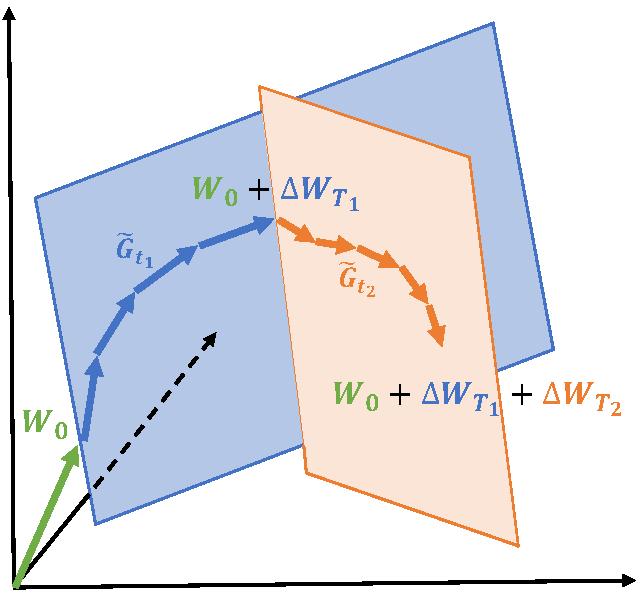
\includegraphics[width=0.58\linewidth]{figures/files/subspace_learning.pdf}
    \caption{\small{ Learning through low-rank subspaces $\Delta W_{T_1}$ and $\Delta W_{T_2}$ using \lowrank{}. For $t_1 \in [0, T_1 - 1]$, $W$ are updated by projected gradients $\tilde G_{t_1}$ in a subspace determined by fixed $P_{t_1}$ and $Q_{t_1}$. After $T_1$ steps, the subspace is changed by recomputing $P_{t_2}$ and $Q_{t_2}$ for $t_2 \in [T_1, T_2 - 1]$, and the process repeats until convergence.}}
    \label{fig:subspace_learning}
\vspace{-3mm}
\end{figure}
